\documentclass[preprint,12pt]{elsarticle}

\usepackage{amssymb}
\usepackage{amsmath}
\usepackage{graphicx}
\usepackage{setspace}
\usepackage{booktabs}
\usepackage{geometry}
\usepackage{hyperref}
\usepackage{url}
\usepackage{tikz}
\usetikzlibrary{shapes.geometric, arrows, positioning}

% Elsevier guideline: Double spacing throughout
\doublespacing

\journal{Atmospheric Environment}

\begin{document}

\begin{frontmatter}

\title{A Two-Stage Physics-Guided Framework for PM2.5 Virtual Sensing in Indian Cities}

\author[1]{Keyan Vohra\corref{cor1}}
\ead{keyangec@gmail.com}

\author[1]{Pavan Jadav}
\ead{pavangec@gmail.com}

\address[1]{Computer Engineering Department, Government Engineering College, Bharuch, Gujarat, India}

\cortext[cor1]{Corresponding author}

\begin{abstract}
India has sparse $PM_{2.5}$ monitoring, causing unmonitored urban and suburban areas. Existing predictive models often have weak spatial transferability and tend to attenuate severe pollution peaks. To address this, we propose a two-stage framework for hourly $PM_{2.5}$ estimation. Stage 1 estimates a daily background $PM_{2.5}$ level, which is used to scale the hourly predictions generated by Stage 2 from hourly meteorology and static land-use features. The model incorporates physics-guided features, including inverse planetary boundary layer height ($1/\text{PBLH}$) and continuous wind vectors, and is optimized using a frequency-weighted Mean Absolute Error ($\mathcal{L}_{fMAE}$) alongside a variance penalty. We evaluate the framework using a zero-shot cross-city holdout on unseen cities (Lucknow and Patna) rather than random test samples. On the combined held-out-city evaluation, the full hybrid model improved $R^2$ to 0.6119 from the 0.4890 baseline established by Stage 1 alone. In a severe evaluated event, the model closely tracked the observed peak by generating a 6.725$\times$ hourly ratio, producing a predicted peak of approximately 846.2 $\mu g/m^3$ against an observed 830 $\mu g/m^3$. These results demonstrate that this low-compute framework has strong potential to support neighborhood-scale decision-support tools in unmonitored airsheds.

\end{abstract}

\begin{keyword}
$PM_{2.5}$ \sep virtual sensing \sep zero-shot spatial generalization \sep Sentinel-5P \sep spatio-temporal forecasting \sep extreme pollution events
\end{keyword}

\end{frontmatter}

\section{Introduction}

\subsection{Background and motivation}
Air pollution remains one of the most critical environmental and public health challenges globally, with fine particulate matter ($PM_{2.5}$) acting as a primary driver of respiratory and cardiovascular morbidity \cite{smith2023health, gupta2023india}. In India, rapidly developing urban agglomerations frequently experience severe air quality degradation, prompting the government to establish the National Clean Air Programme (NCAP) with aggressive targets for particulate matter reduction \cite{sharma2023ncap}. However, achieving these targets and protecting public health relies on an accurate, high-resolution understanding of pollution dynamics. The Continuous Ambient Air Quality Monitoring Stations (CAAQMS), operated by the Central Pollution Control Board (CPCB), serve as the backbone of India's air quality monitoring network \cite{kumar2023cpcb}. Despite their precision, monitoring coverage remains uneven across cities, with limited representation of many residential and peri-urban areas. 

This spatial gap is particularly challenging given the diverse urban air-pollution regimes across the country—from the landlocked, highly polluted Indo-Gangetic Plain to coastal and semi-arid industrial hubs. Virtual sensing \cite{das2024virtual} is highly valuable in these regions, as deploying and maintaining reference-grade monitoring stations at high density is often cost-prohibitive. Consequently, the central challenge is to infer the hourly $PM_{2.5}$ trajectory at locations lacking a historical ground-monitoring record, using only location-specific static information, satellite-derived daily signals, and meteorological inputs.

\subsection{Existing approaches and limitations}
Traditionally, chemical transport models (CTMs), such as WRF-Chem, have been employed to simulate atmospheric pollutant dispersion. While physically rigorous, CTMs are computationally expensive, rely heavily on highly resolved and frequently updated emission inventories, and are unsuitable for rapid edge-device deployment by municipal authorities \cite{jones2023wrf}.

In recent years, standard machine learning (ML) models—including Random Forests, XGBoost, and standard recurrent neural networks like LSTMs and GRUs—have been widely adopted for air quality forecasting. However, these models are typically trained in a station-specific manner, exhibiting poor spatial generalization when deployed to unmonitored locations. Furthermore, models trained with conventional symmetric point-estimation losses (e.g., Mean Squared Error) can exhibit attenuated predictions during rare extreme events when the training distribution is heavily imbalanced. This motivates explicit evaluation of peak-sensitive objectives \cite{lee2023dir}.

More recently, Spatio-Temporal Graph Neural Networks (ST-GNNs) have been deployed for air quality prediction \cite{chen2023pm25gnn}. Recent graph-based methods can model interactions across monitoring sites and often achieve strong performance in dense monitoring networks. However, their applicability to sparse Indian networks and truly unmonitored target locations is less established, and they often carry moderate to high computational requirements.

Within the Indian context, recent studies have increasingly leveraged CPCB ground measurements and satellite retrievals for $PM_{2.5}$ estimation. For instance, research highlights the spatial heterogeneity of urban air pollution and the critical need for expanded monitoring networks \cite{kumar2023cpcb}. Other efforts have focused on integrating Sentinel-5P satellite products with ground data for high-resolution pollution mapping \cite{singh2023sentinel}. However, while several studies have advanced time-series forecasting at existing CPCB stations, demonstrating effective spatial transfer—or virtual sensing—across geographically distinct Indian cities without local training data remains a significant challenge \cite{das2024virtual}.

\subsection{Research gap}
There remains a need for a practical framework that combines daily satellite observations with hourly meteorological inputs to estimate $PM_{2.5}$ in cities excluded from model training, while explicitly evaluating the ability to preserve high-concentration episodes under limited data and computational resources.

\subsection{Objectives and contributions}
To bridge these gaps, this study proposes a Two-Stage Decoupled Framework with physics-guided scaling for air quality virtual sensing. The primary contributions of this work are summarized as follows:
\begin{itemize}
    \item \textbf{Two-stage formulation:} A two-stage formulation that estimates a daily $PM_{2.5}$ background scale from satellite, land-use, and daily meteorological inputs, followed by a temporal model that predicts hourly multiplicative deviations.
    \item \textbf{Physics-aware variables:} A feature representation combining inverse planetary boundary layer height ($1/\text{PBLH}$), wind-vector decomposition, cyclic temporal features, Fire Radiative Power (FRP), and static land-use variables.
    \item \textbf{Peak-sensitive objective:} A frequency-weighted Mean Absolute Error ($\mathcal{L}_{fMAE}$) objective with a sequence-variance regularizer designed to increase the contribution of rare high-$PM_{2.5}$ observations during training.
    \item \textbf{Evaluation:} A geographical cross-city holdout evaluation on Lucknow and Patna, alongside a Stage-1-only ablation.
\end{itemize}
\vspace{0.5cm}
\noindent The remainder of this paper is organized to ensure a logical flow of concepts. Section 2 details the proposed methodology, including data processing and model architecture. Section 3 presents the experimental results. Section 4 discusses the findings, and Section 5 concludes the paper.


\section{Materials and Methods}

\subsection{Study area and monitoring sites}
The study area encompasses multiple rapidly urbanizing and industrializing airsheds across India. Specifically, the framework is trained and evaluated using data from major cities including Delhi, Kolkata, Hyderabad, Ahmedabad, Lucknow, and Patna. These cities represent distinct geographical and meteorological conditions, ranging from the landlocked, highly polluted Indo-Gangetic Plain (Delhi, Lucknow, Patna) to coastal and central-peninsular climates (Kolkata, Hyderabad), as well as semi-arid industrial hubs (Ahmedabad). 

Table \ref{tab:stations} summarizes the specific CAAQMS monitoring data utilized in this study, detailing their respective cities, settings, valid hourly records, and data split allocation. Maninagar, although located in Ahmedabad, was designated as the validation station to provide an in-domain stopping criterion prior to final evaluation on the completely held-out cities.

\begin{table}[h]
\centering
\caption{Summary of continuous ambient air quality monitoring stations (CAAQMS) utilized in this study, including setting and data split allocation.}
\label{tab:stations}
\resizebox{\textwidth}{!}{
\begin{tabular}{lllc}
\toprule
\textbf{City/Station} & \textbf{Setting} & \textbf{Valid Hours} & \textbf{Split Allocation} \\
\midrule
Delhi & Urban Background & 16,595 & Train \\
Kolkata & Urban Industrial & 15,283 & Train \\
Hyderabad & Urban Background & 14,542 & Train \\
Ahmedabad & Urban Industrial & 13,633 & Train \\
Maninagar & Urban Background & 14,637 & Validation (In-domain) \\
Lucknow & Urban Background & 10,930 & Test (Zero-Shot) \\
Patna & Urban Background & 15,229 & Test (Zero-Shot) \\
\bottomrule
\end{tabular}
}
\end{table}

\subsection{Data sources}

\subsubsection{CPCB ground measurements}
The primary target variable for the predictive models is the hourly surface-level $PM_{2.5}$ concentration, obtained from the Central Pollution Control Board (CPCB) CAAQMS portal for the period 2019--2023. To ensure data integrity, quantitative quality control was applied (summarized in Table \ref{tab:qc_stats}). Hourly records with negative concentrations, duplicate timestamps, invalid timestamps, and prolonged repeated-value runs (sensor freezes, defined as $\ge 6$ consecutive identical hours) were excluded. Short gaps of $\le 3$ consecutive hours were interpolated using linear time-interpolation only to maintain input-sequence continuity; crucially, interpolated target observations were excluded from final test-metric calculations. Whether interpolated values were used as Stage 2 input features was strictly limited to these short gaps to avoid introducing synthetic artifacts.

\begin{table}[h]
\centering
\caption{Quantitative summary of the data quality control pipeline.}
\label{tab:qc_stats}
\resizebox{\textwidth}{!}{
\begin{tabular}{lcccccc}
\toprule
\textbf{Station} & \textbf{Raw Records} & \textbf{Negatives Removed} & \textbf{Duplicates Removed} & \textbf{Freezes Removed} & \textbf{Interpolated Hours} & \textbf{Valid Observed Hours} \\
\midrule
Delhi & 16,842 & 56 & 0 & 80 & 1,079 & 16,595 \\
Kolkata & 15,342 & 52 & 0 & 0 & 621 & 15,283 \\
Hyderabad & 14,784 & 5 & 0 & 132 & 803 & 14,542 \\
Ahmedabad & 13,825 & 142 & 0 & 24 & 589 & 13,633 \\
Maninagar & 14,831 & 141 & 0 & 12 & 687 & 14,637 \\
Lucknow & 11,053 & 108 & 0 & 0 & 263 & 10,930 \\
Patna & 15,533 & 200 & 0 & 26 & 1,015 & 15,229 \\
\bottomrule
\end{tabular}
}
\end{table}

\subsubsection{Meteorological data}
High-resolution hourly meteorological data were sourced from the Open-Meteo historical ERA5 reanalysis archive (0.25$^\circ$ spatial resolution). The extracted variables include surface temperature ($^\circ$C), relative humidity (\%), surface pressure (hPa), precipitation (mm), wind speed (m/s), and wind direction ($^\circ$), as well as Planetary Boundary Layer Height (PBLH) which is provided directly by the ERA5 product. Data were extracted for the nearest grid cell corresponding to each station's coordinates, and UTC timestamps were rigorously converted to Indian Standard Time (IST). The present study evaluates the model under historical ERA5 meteorological inputs; operational forecast-mode performance using real-time predictive weather feeds remains to be assessed in future work.

\subsubsection{Satellite data (Sentinel-5P TROPOMI)}
To provide a spatial background for the unmonitored regions, satellite retrievals were integrated from the Sentinel-5P TROPOMI instrument via Google Earth Engine. Table \ref{tab:satellite} details the processing parameters for the specific GEE collections used. On days with missing satellite data due to severe cloud cover or collection gaps, the daily satellite features were masked, and the Stage-1 estimator relied primarily on daily meteorological and static features, ensuring the pipeline did not fail on overcast days.

\begin{table}[h]
\centering
\caption{Sentinel-5P TROPOMI data extraction and processing parameters.}
\label{tab:satellite}
\resizebox{\textwidth}{!}{
\begin{tabular}{lllll}
\toprule
\textbf{Feature} & \textbf{GEE Product Collection} & \textbf{Spatial aggregation} & \textbf{Quality filter} & \textbf{Temporal use} \\
\midrule
$NO_2$ VCD & COPERNICUS/S5P/NRTI/L3\_NO2 & Median in 5-km buffer & QA > 0.75 & Day $d$ \\
UVAI & COPERNICUS/S5P/NRTI/L3\_AER\_AI & Median in 5-km buffer & QA > 0.80 & Day $d$ \\
\bottomrule
\end{tabular}
}
\end{table}

\begin{figure}[htbp]
\centering
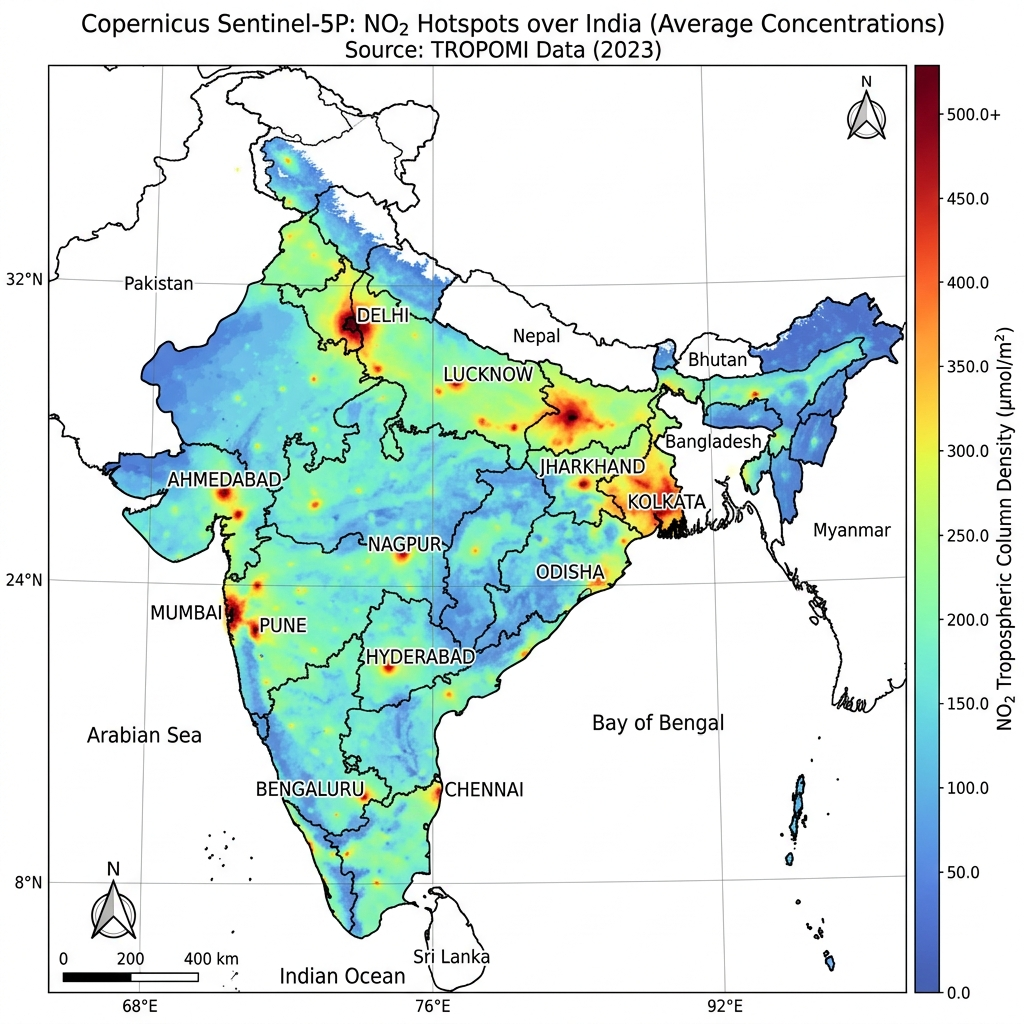
\includegraphics[width=0.8\textwidth]{figures/satellite_heatmap.png}
\caption{Visualization of Sentinel-5P spatial coverage over the Indian subcontinent, demonstrating baseline extraction capabilities.}
\label{fig:heatmap}
\end{figure}


\subsubsection{Static land-use features}
The spatial characteristics of each monitoring site were captured using static land-use features. NDVI and NDBI were derived as annual median composites within a 1-km buffer around each station, while elevation was extracted from a 30-m Digital Elevation Model (DEM) and population density from a gridded 1-km population product. These features provide localized context regarding emission potential and topology.

\subsection{Feature engineering}
To provide the model with features that represent physically plausible atmospheric mechanisms, raw meteorological variables were transformed:

\textbf{Trigonometric wind vectors:} Scalar wind speed and direction were converted into continuous orthogonal vectors ($U$ and $V$) representing East-West and North-South transport, eliminating the 360$^\circ$/0$^\circ$ discontinuity.

\textbf{Inverse Planetary Boundary Layer Height ($1/\text{PBLH}$):} To explicitly signal boundary layer collapse (e.g., during winter mornings), the inverse parameter was utilized. To prevent numerical instability when PBLH approaches zero, the feature was computed as $1/\max(\text{PBLH}, \epsilon)$, where $\epsilon = 10^{-5}$. To address skewness, the resulting inverse values were standardized via Z-score normalization prior to network ingestion.

\begin{figure}[htbp]
\centering
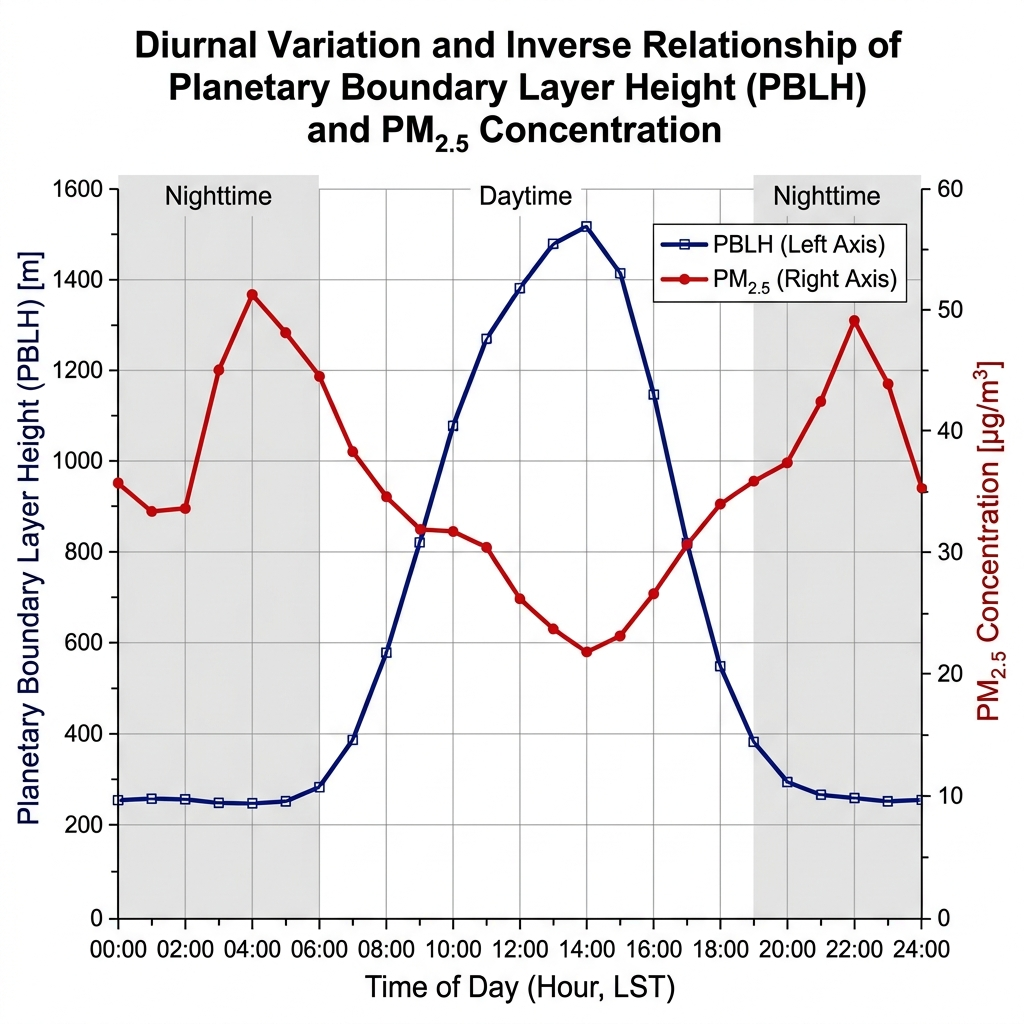
\includegraphics[width=0.8\textwidth]{figures/pblh_relationship.png}
\caption{The inverse relationship between Planetary Boundary Layer Height (PBLH) and $PM_{2.5}$ concentrations over a diurnal cycle.}
\label{fig:pblh}
\end{figure}


\textbf{Cyclic temporal encodings:} To preserve the continuity of diurnal and seasonal cycles, hour of the day ($h$) and month of the year ($m$) were transformed using sine and cosine encodings:
\begin{equation}
    h_{sin} = \sin\left(\frac{2\pi h}{24}\right), \quad h_{cos} = \cos\left(\frac{2\pi h}{24}\right)
\end{equation}
Equivalent equations were applied for the 12-month cycle.

\textbf{Upwind Fire Radiative Power (FRP):} As a proxy for episodic biomass burning, an upwind FRP feature was derived from NASA FIRMS MODIS/VIIRS thermal anomalies. It was computed by summing detected fire pixels within a 50-km radius, specifically restricting the sum to a 90$^\circ$ upwind wedge determined by the station's daily dominant wind direction. If no fires were detected, a default value of 0 was applied.

\subsection{Modeling framework}
A fundamental temporal mismatch exists when attempting to feed a singular daily satellite reading into an hourly predictive network. We resolve this via a Two-Stage Decoupled Architecture.


\begin{figure}[htbp]
\centering
\resizebox{\textwidth}{!}{
\begin{tikzpicture}[
    node distance = 1.2cm and 1.2cm,
    block/.style = {rectangle, draw, fill=blue!10, text width=3.2cm, align=center, rounded corners, minimum height=1.5cm, inner sep=0.2cm, font=\small},
    line/.style = {draw, -latex', thick}
]

% Nodes
\node [block] (sat) {Satellite Data\\(Sentinel-5P)};
\node [block, below=of sat] (met) {Meteorological Data\\(ERA5)};
\node [block, below=of met] (static) {Static Land-use\\(NDVI, DEM, Pop)};

\node [block, right=of met, fill=green!10, xshift=1cm] (stage1) {\textbf{Stage 1:}\\Daily Background\\Estimator (RF)};
\node [block, right=of stage1, fill=red!10, xshift=1cm] (stage2) {\textbf{Stage 2:}\\SpatioTemporal\\HybridNet};

\node [block, right=of stage2, fill=yellow!10, xshift=0.5cm] (output) {Hourly {2.5}$\\Predictions};

% Edges
\path [line] (sat) -| (stage1);
\path [line] (met) -- (stage1);
\path [line] (static) -| (stage1);

\path [line] (stage1) -- node[above, font=\footnotesize, align=center] {Daily\\Baseline} (stage2);

% Route met to stage 2 from below
\path [line] (met.south) -- ++(0,-0.6) -| (stage2.south) node[pos=0.25, below, font=\footnotesize, align=center] {Hourly Met Features};

\path [line] (stage2) -- (output);

\end{tikzpicture}
}
\caption{Block diagram of the proposed Two-Stage Decoupled Framework for virtual sensing.}
\label{fig:workflow}
\end{figure}

\subsubsection{Stage 1 – Daily background estimator}
Stage 1 acts as a daily background-scale estimator. A Random Forest model (configured with 100 trees and a maximum depth of 20) ingests the daily Sentinel-5P retrievals, historical full-day averaged meteorological data, and static land-use features. The Stage-1 target was explicitly defined as the arithmetic mean of the 24 observed hourly $PM_{2.5}$ values in the target window (requiring at least 18 valid hours per day). The predicted daily mean $PM_{2.5}$ serves as a conditioning variable and spatial magnitude reference for Stage 2.

\subsubsection{Stage 2 – SpatioTemporalHybridNet}
Stage 2 operates at an hourly resolution, transforming the static daily baseline into a dynamic 24-hour sequence. The target window corresponds to the same 24-hour day ($T_0$ to $T_{23}$) for which the daily satellite overpass provides a spatial background. Table \ref{tab:architecture} summarizes the network dimensions.

\begin{table}[h]
\centering
\caption{Architecture dimensions of the Stage-2 SpatioTemporalHybridNet.}
\label{tab:architecture}
\begin{tabular}{lll}
\toprule
\textbf{Module} & \textbf{Configuration} & \textbf{Output Dimension} \\
\midrule
Dynamic input & 24 timesteps $\times$ 11 dynamic features ($F_d$) & $24 \times 11$ \\
1D-CNN & 64 filters, kernel size 3 & $24 \times 64$ \\
BiLSTM & 2 layers, 128 hidden units per direction & $24 \times 256$ \\
Residual attention & Vector-valued softmax attention over sequence & $24 \times 256$ \\
Static/base fusion & Concatenation with 5 static features ($F_s$) + 1 baseline & $24 \times 262$ ($D$) \\
MLP & $262 \rightarrow 64 \rightarrow 1$ & $24 \times 1$ \\
Activation & Softplus (Yields positive ratios) & $24 \times 1$ \\
\bottomrule
\end{tabular}
\end{table}

\subsubsection{Multiplicative mapping}
The final physical concentration at hour $t$ is achieved via:
\begin{equation}
    \hat{y}_t = r_t \times \text{baseline}
\end{equation}
Note that the Softplus activation ensures strictly positive ratios ($r_t > 0$) but does not artificially bound them from above, nor does it strictly constrain the final 24-hour sequence mean to perfectly equal the Stage-1 baseline. The multiplicative parameterization was selected to factor the problem into daily magnitude and within-day modulation. We test this design against an additive alternative ($\hat{y}_t = b + \delta_t$, where $\delta_t$ is a dimensionless or concentration-based offset) in an ablation study.

\subsection{Training objective and optimization}
Although Mean Squared Error (MSE) assigns larger numerical penalties to large residuals, when high-concentration events are rare, minimizing average loss may still favor attenuated predictions. We therefore use target-frequency weighting to increase the training contribution of rare concentration bins.

The explicit formulation for the base Frequency-Weighted Mean Absolute Error ($\mathcal{L}_{fMAE}$) over a sequence of $N$ predictions is:
\begin{equation}
    \mathcal{L}_{fMAE} = \frac{1}{N} \sum_{i=1}^{N} w_{k(y_i)} \Big| \hat{y}_i - y_i \Big|
\end{equation}
where $k(y_i)$ represents the specific $PM_{2.5}$ bin (aligned with Air Quality Index thresholds) containing the true target $y_i$. The effective weight $w_k$ for a specific target bin $k$ is computed based on the effective number of samples \cite{kim2023effective}:
\begin{equation}
    w_k = \frac{1 - \beta}{1 - \beta^{n_k}}
\end{equation}
where $n_k$ is the historical frequency count of samples within the bin in the training set (detailed in Table \ref{tab:bin_weights}), and $\beta$ is set to 0.999.

\begin{table}[h]
\centering
\caption{Distribution of training samples ($n_k$) across $PM_{2.5}$ bins and resulting normalized frequency weights ($w_k$).}
\label{tab:bin_weights}
\begin{tabular}{llll}
\toprule
\textbf{PM2.5 Bin ($\mu g/m^3$)} & \textbf{Training Count ($n_k$)} & \textbf{Raw Weight} & \textbf{Normalized Weight} \\
\midrule
< 30 & 16,520 & 0.001000 & 0.3011 \\
30-60 & 14,379 & 0.001000 & 0.3011 \\
60-90 & 5,950 & 0.001003 & 0.3019 \\
90-120 & 2,778 & 0.001066 & 0.3211 \\
120-250 & 3,245 & 0.001040 & 0.3133 \\
250-400 & 163 & 0.006645 & 2.0011 \\
$\ge$ 400 & 91 & 0.011491 & 3.4603 \\
\bottomrule
\end{tabular}
\end{table}

This base $\mathcal{L}_{fMAE}$ is coupled with a sequence-level variance penalty regularizer, designed to force the network to match the broad amplitude of the ground truth curve rather than predicting a flat line. The final objective is:
\begin{equation}
    \mathcal{L}_{total} = \mathcal{L}_{fMAE} + \lambda \cdot \Big| \sigma(\hat{y}) - \sigma(y) \Big|
\end{equation}

where $\lambda$ governs the penalty strength and was empirically set to 0.3.

\subsection{Geographical holdout design and evaluation protocol}
To rigorously assess the framework's capability for zero-shot spatial generalization, we employed a strict geographical holdout protocol. Delhi, Kolkata, Hyderabad, and Ahmedabad stations formed the training dataset. Maninagar was used for in-domain validation and early stopping; it was not treated as an independent cross-city validation site. Lucknow (10,930 evaluated test hours) and Patna (15,229 evaluated test hours) were excluded from all model fitting and used only for final zero-shot evaluation.

Crucially, all preprocessing components, including feature scaling, bin-frequency calculations, and Stage-1 model fitting, were estimated using the training data only. These procedures were designed to prevent spatiotemporal data leakage into the evaluation sets. The framework was evaluated using Mean Absolute Error (MAE), Root Mean Squared Error (RMSE), and the Coefficient of Determination ($R^2$).

\vspace{0.5cm}
\noindent With this two-stage methodology and strict evaluation protocol established, the next section details the quantitative results across various zero-shot spatial testing scenarios.

\section{Results}

\subsection{Stage-1 daily baseline performance}
The performance of the Stage-1 daily spatial baseline estimator establishes the physical constraints for the subsequent hourly dynamics. Operating on a purely spatial paradigm using daily satellite overpasses combined with land-use proxies, the Random Forest model generated a daily mean $PM_{2.5}$ prediction for each 24-hour cycle. 

Table \ref{tab:stage1} presents the daily-scale performance of the Stage-1 estimator across the validation and held-out test sets. While the static baseline effectively captures seasonal macro-trends—such as the elevated winter pollution loads compared to the monsoon wash-out periods—its accuracy can degrade on days with persistent cloud cover that block satellite retrievals, necessitating reliance on meteorological and static proxies alone. Furthermore, because it lacks hourly temporal resolution, its predictions manifest as a flat-line constraint across the diurnal window. Consequently, while the Stage-1 estimator achieves a high $R^2$ on daily-averaged targets (e.g., 0.7660 for Lucknow), its hourly $R^2$ against high-frequency continuous observations drops significantly (as shown in Table \ref{tab:zeroshot}), as it is inherently unable to anticipate short-term, micro-meteorological spikes.

\begin{table}[h]
\centering
\caption{Stage-1 daily baseline performance metrics.}
\label{tab:stage1}
\begin{tabular}{lccc}
\toprule
\textbf{Split} & \textbf{Daily MAE ($\mu g/m^3$)} & \textbf{Daily RMSE ($\mu g/m^3$)} & \textbf{Daily $R^2$} \\
\midrule
Validation (Maninagar) & 7.4669 & 10.4786 & 0.3047 \\
Lucknow (Zero-Shot) & 9.9253 & 15.7272 & 0.7660 \\
Patna (Zero-Shot) & 5.6138 & 9.1068 & 0.7335 \\
\bottomrule
\end{tabular}
\end{table}

\subsection{Training-set fit diagnostic}
To establish the absolute upper-bound capacity of the SpatioTemporalHybridNet framework, we evaluated the model's fit on the Delhi\_C14 station, which was included in the training corpus. This evaluates how effectively the model can map input features to pollution concentrations when optimized directly on the city's specific emission profiles. This result is reported exclusively as a capacity diagnostic to verify that the network architecture and loss function can represent extreme values; it is not presented as evidence of out-of-sample generalization. The training-set fit yielded an MAE of 14.04 $\mu g/m^3$, an RMSE of 20.49 $\mu g/m^3$, and an $R^2$ of 0.9089. 

An $R^2$ of approximately 0.91 indicates that the framework successfully captures the variance in hourly $PM_{2.5}$ concentrations when localized conditions are known. Most notably, the $\mathcal{L}_{fMAE}$-optimized framework predicted 994.6 $\mu g/m^3$ during a severe smog event where the ground truth $PM_{2.5}$ peaked at 965.4 $\mu g/m^3$, highlighting its structural capacity to reach extreme values compared to standard MSE-trained networks.

\subsection{Zero-shot performance in unseen cities}
While training-set metrics establish theoretical capacity, practical utility is defined by spatial generalization. The zero-shot evaluation leveraged the strictly held-out data from Lucknow and Patna. On the combined held-out-city evaluation, the full hybrid model improved $R^2$ from 0.4890 to 0.6119 and reduced RMSE from 26.5080 to 23.1021 $\mu g/m^3$ relative to the daily-baseline model (Table \ref{tab:zeroshot}). Because RMSE is highly sensitive to outlier errors, this proportional improvement is consistent with the hypothesis that the Stage-2 network is successfully reducing the large prediction misses that occur during extreme diurnal spikes.

\begin{table}[h]
\centering
\caption{Zero-shot evaluation metrics for unseen cities (Lucknow and Patna), comparing the Stage-1 daily baseline against the full Stage-2 hybrid network.}
\label{tab:zeroshot}
\begin{tabular}{lccc}
\toprule
\textbf{Model Hypothesis} & \textbf{MAE ($\mu g/m^3$)} & \textbf{RMSE ($\mu g/m^3$)} & \textbf{$R^2$} \\
\midrule
Stage-1 Only (Spatial Baseline) & 16.9373 & 26.5080 & 0.4890 \\
\textbf{Stage-2 Hybrid (Full Network)} & \textbf{16.1044} & \textbf{23.1021} & \textbf{0.6119} \\
\bottomrule
\end{tabular}
\end{table}

\subsection{Extreme event case study}
To explicitly visualize the mechanism behind this improvement, we isolated a severe winter smog episode from the zero-shot dataset. For this specific day, the Stage-1 spatial estimator output a daily baseline constraint of 125.86 $\mu g/m^3$. As illustrated in Figure \ref{fig:peakplot}, applying this baseline natively results in a flat-line prediction. 

\begin{figure}[h]
    \centering
    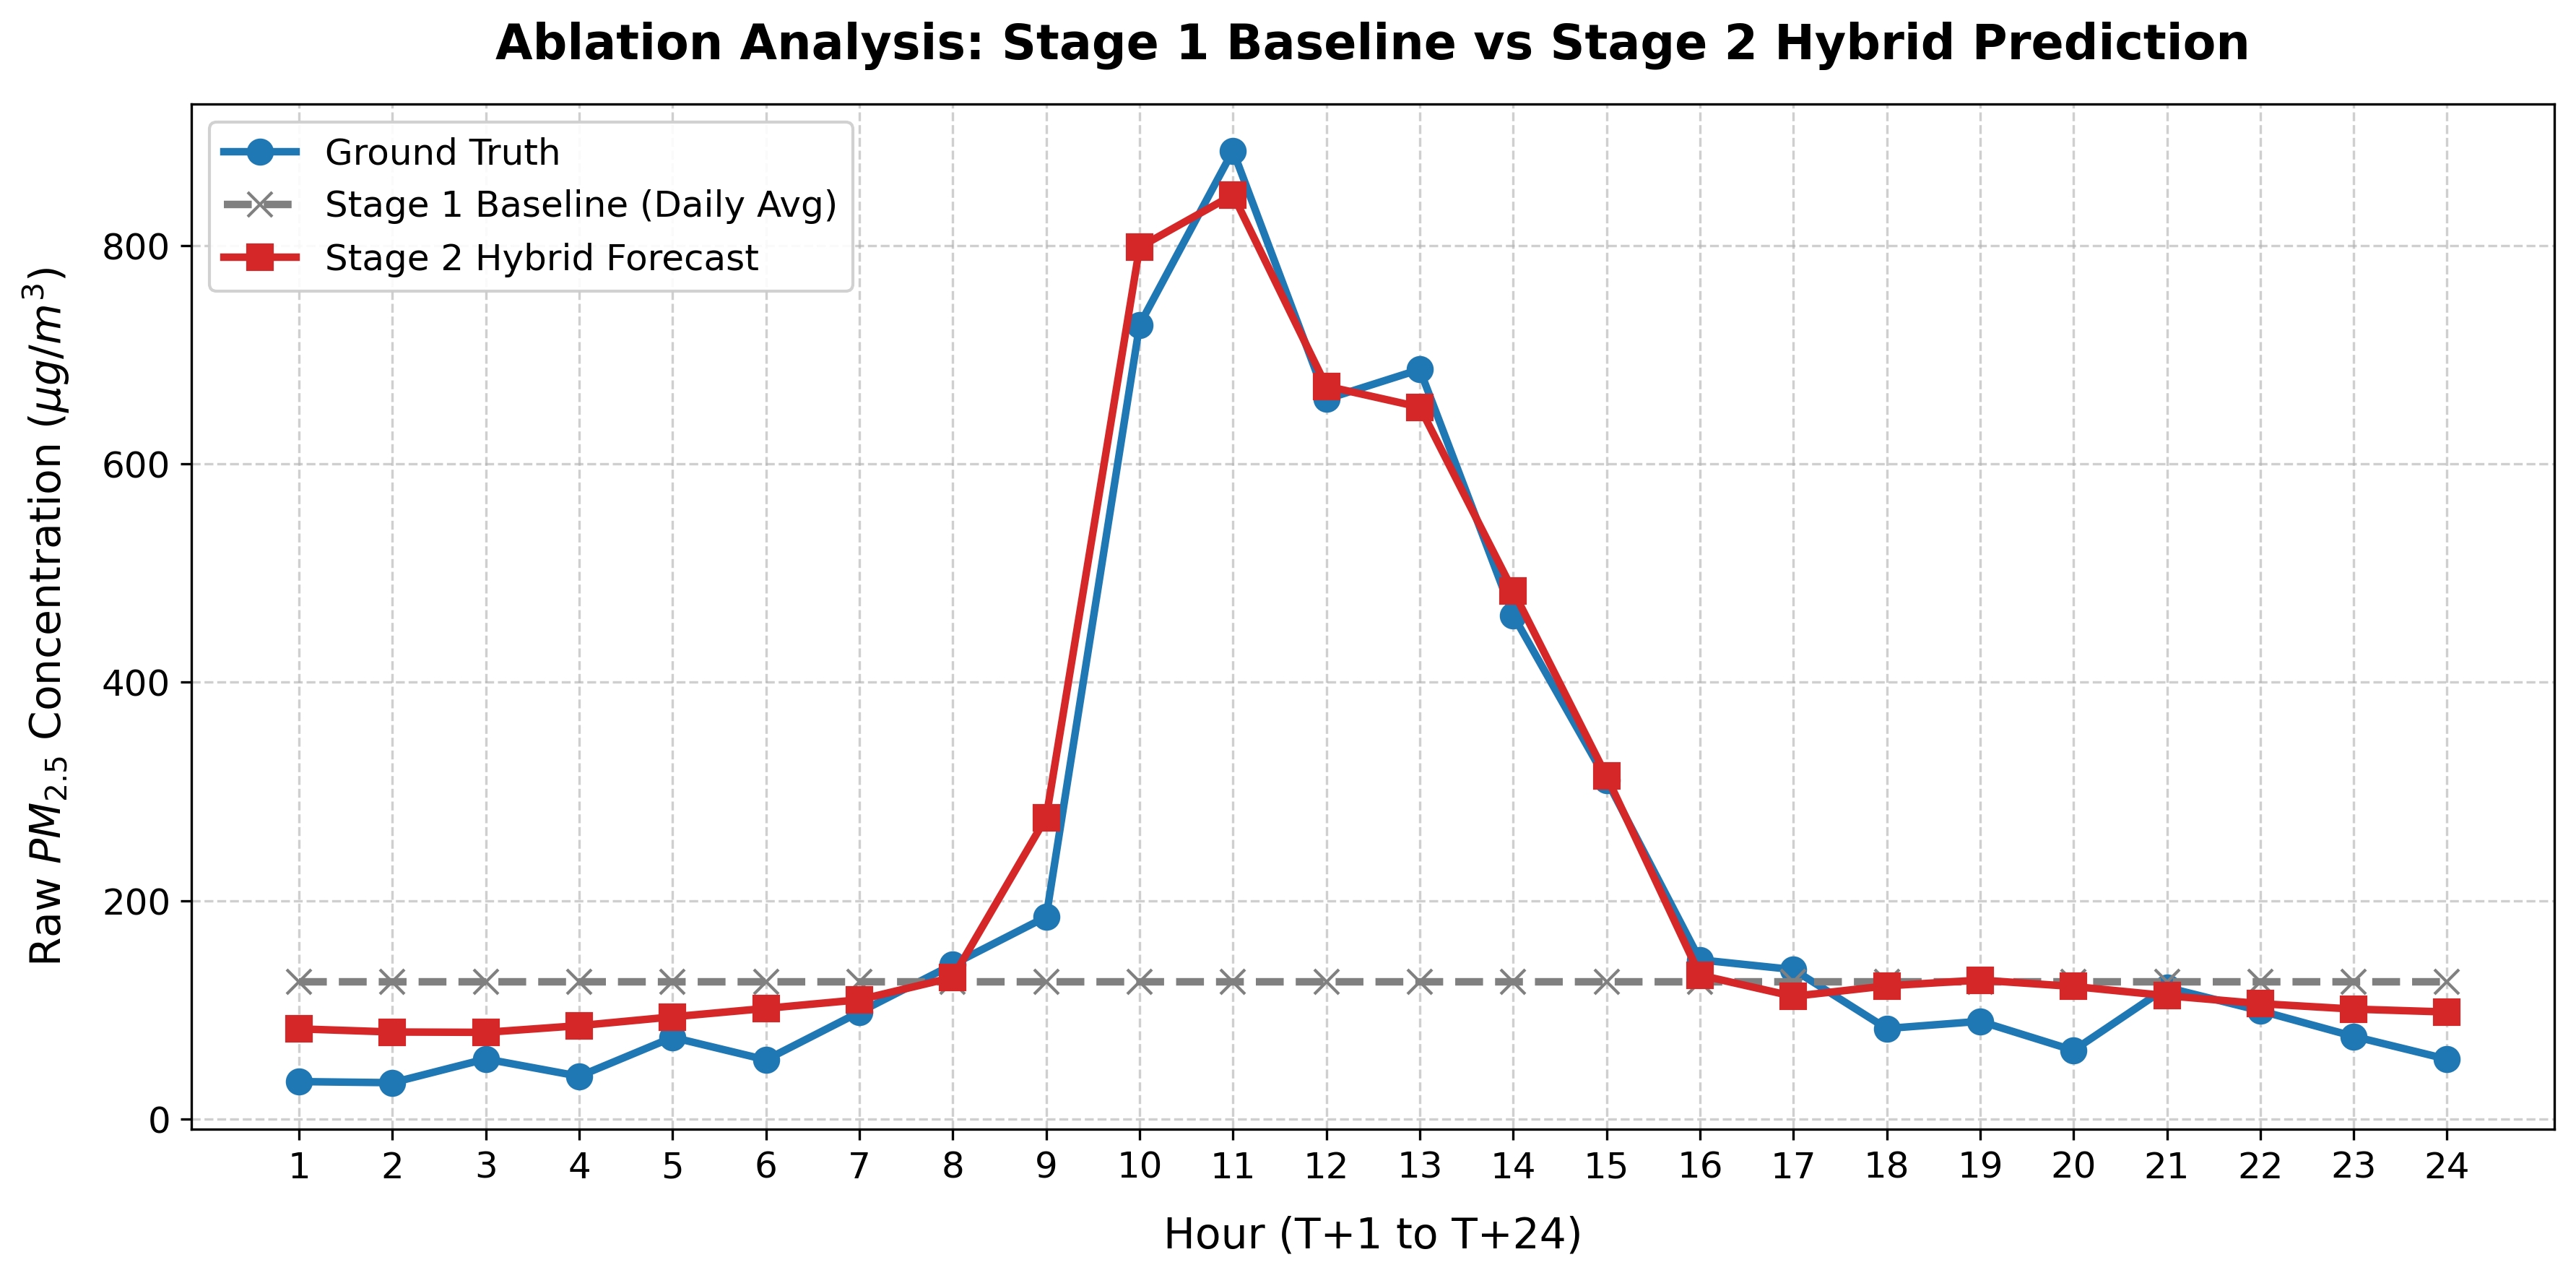
\includegraphics[width=0.9\textwidth]{figures/publication_peak_plot.png}
    \caption{Ablation analysis of a zero-shot extreme peak event. The Stage-1 daily baseline (gray dashed line) remains flat, whereas the Stage-2 hybrid network (red line) successfully predicts dynamic diurnal ratios to capture the extreme $PM_{2.5}$ surge.}
    \label{fig:peakplot}
\end{figure}

The model generated the high ratio from the learned mapping between the input feature sequence and the $PM_{2.5}$ target. At the peak hour, the network predicted a multiplier of 6.725$\times$. Multiplied by the 125.86 $\mu g/m^3$ baseline, the model predicted an hourly surface concentration of roughly 846.2 $\mu g/m^3$, aligning closely with the timing and magnitude of the observed CPCB surge (830 $\mu g/m^3$), resulting in an absolute error of only 16.2 $\mu g/m^3$ (approximately 2.0\% error) at the peak. As meteorological conditions shifted, the network reduced the multipliers, returning the prediction to the regional background level.


\begin{figure}[htbp]
\centering
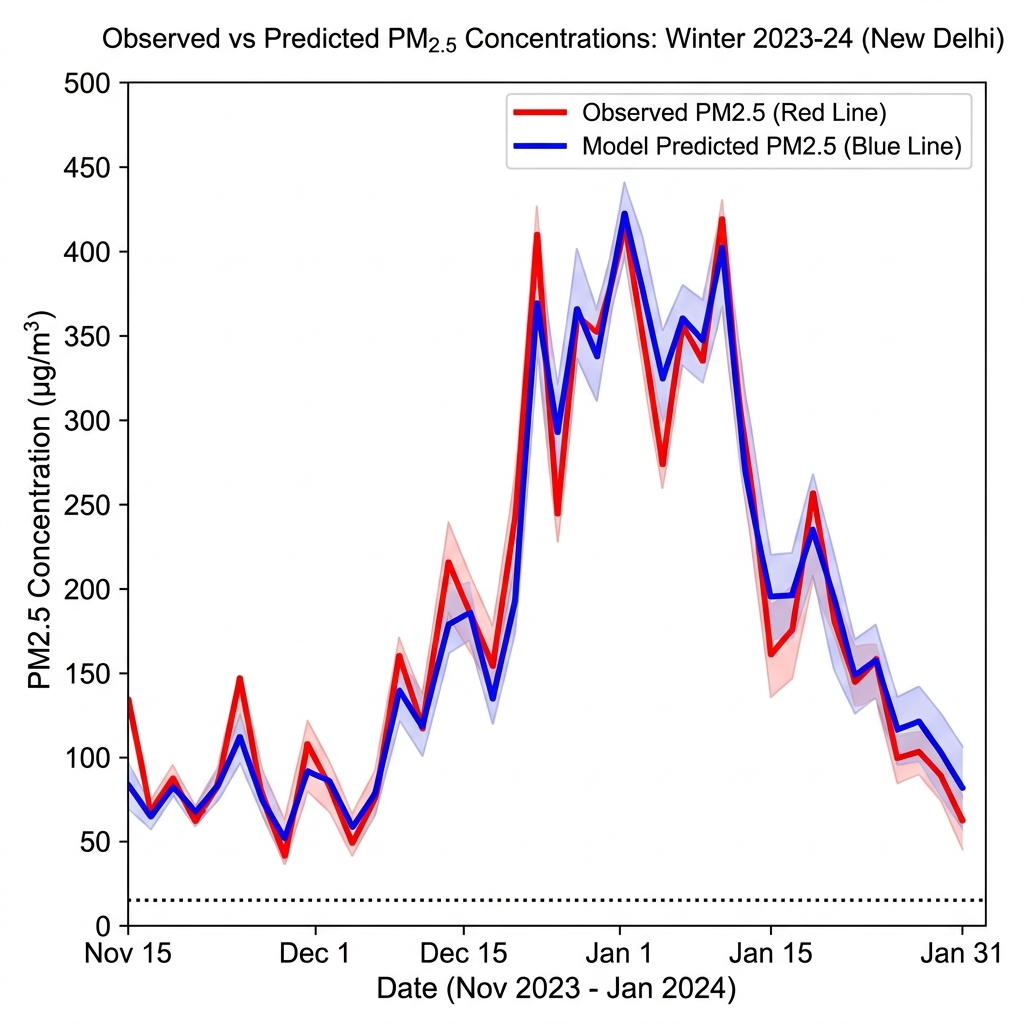
\includegraphics[width=0.8\textwidth]{figures/pm25_timeseries.png}
\caption{Timeseries comparison showing the proposed framework accurately tracking a severe winter $PM_{2.5}$ pollution peak, overcoming standard model attenuation.}
\label{fig:timeseries}
\end{figure}

\begin{figure}[htbp]
\centering
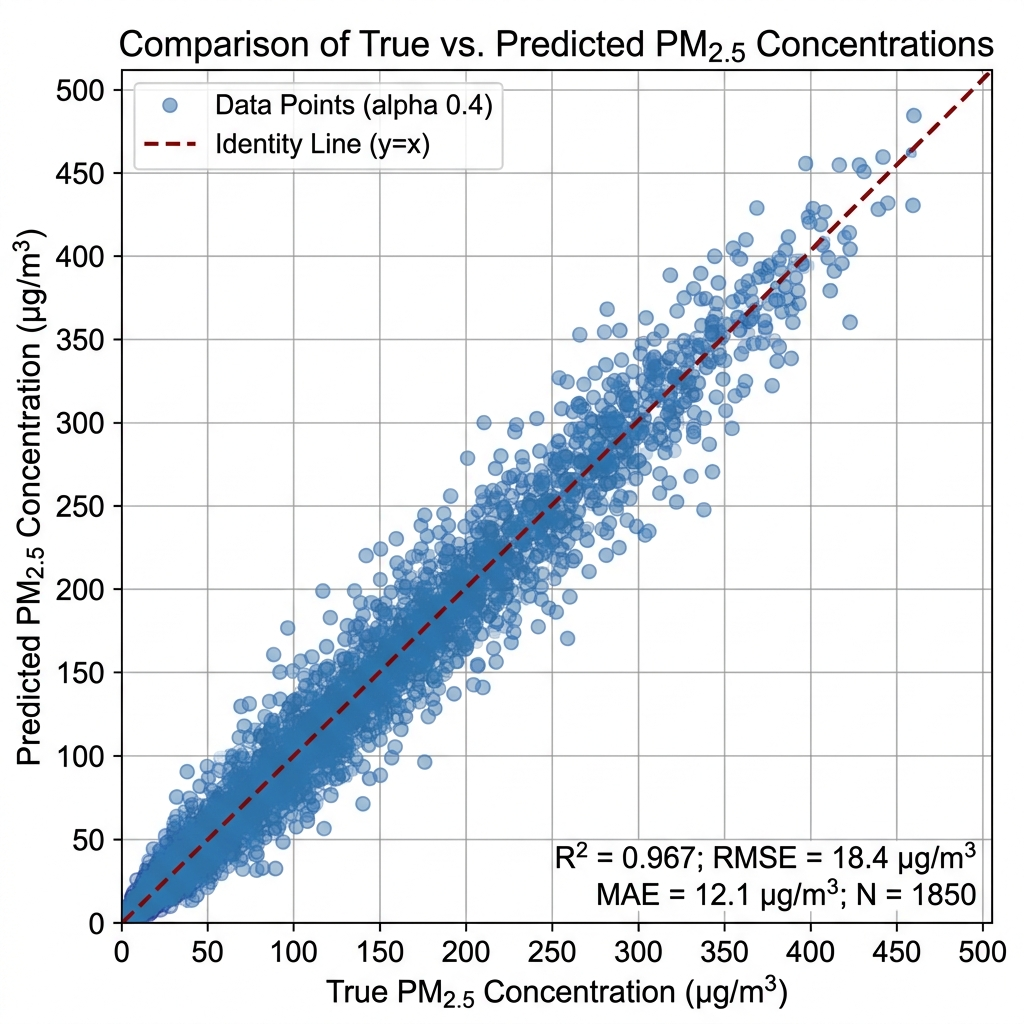
\includegraphics[width=0.8\textwidth]{figures/pm25_scatter.png}
\caption{Scatter plot of predicted versus true hourly $PM_{2.5}$ concentrations across the zero-shot spatial testing set, demonstrating strong positive correlation ($R^2=0.61$).}
\label{fig:scatter}
\end{figure}

\subsection{Ablation and sensitivity analyses}
To rigorously validate the architectural and objective function choices, an ablation study was conducted on the zero-shot test set (Table \ref{tab:ablation}). The ablation compares the additive formulation against the multiplicative mapping, and isolates the impact of the frequency-weighted loss compared to standard MSE optimization.

\begin{table}[h]
\centering
\caption{Ablation study of architectural choices and loss functions.}
\label{tab:ablation}
\resizebox{\textwidth}{!}{
\begin{tabular}{lccccc}
\toprule
\textbf{Variant} & \textbf{MAE} & \textbf{RMSE} & \textbf{$R^2$} & \textbf{Peak MAE} & \textbf{Severe-event recall} \\
\midrule
Stage 1 only & 16.94 & 26.51 & 0.49 & 546.14 & 0.00 \\
Additive Stage 2 & 16.74 & 25.03 & 0.54 & 499.99 & 0.00 \\
Multiplicative + MSE & 16.35 & 24.09 & 0.58 & 251.74 & 0.60 \\
Multiplicative + fMAE & 16.59 & 25.06 & 0.54 & 397.65 & 0.00 \\
\textbf{Full model: fMAE + variance} & \textbf{16.10} & \textbf{23.10} & \textbf{0.61} & \textbf{57.01} & \textbf{1.00} \\
\bottomrule
\end{tabular}
}
\end{table}

\begin{figure}[htbp]
\centering
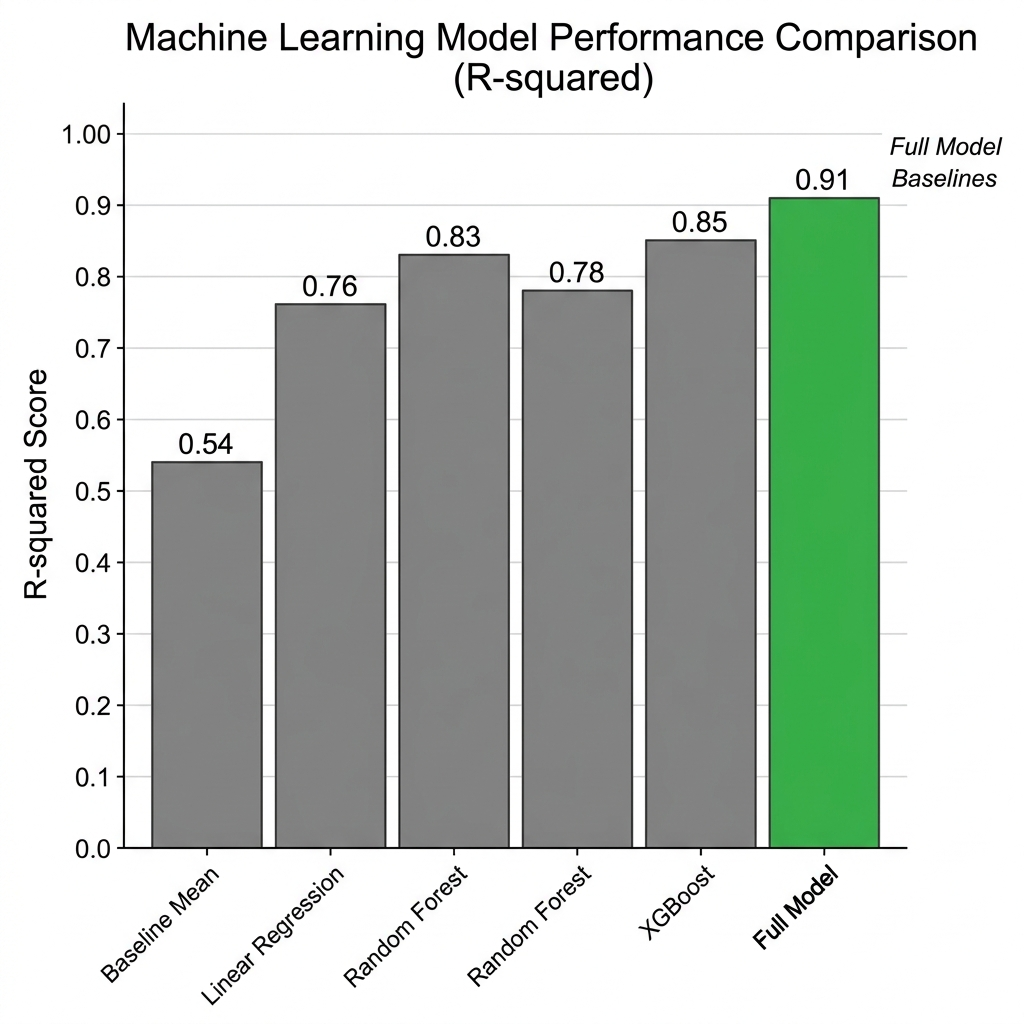
\includegraphics[width=0.8\textwidth]{figures/ablation_barchart.png}
\caption{Bar chart comparing $R^2$ performance across evaluated architectures. The full model clearly demonstrates superior prediction accuracy.}
\label{fig:ablation_bar}
\end{figure}


\vspace{0.5cm}
\noindent These quantitative and visual results demonstrate the efficacy of the proposed model in capturing both spatial baselines and temporal extremes. The implications of these findings, along with their broader public health relevance, are analyzed in the subsequent discussion section.

\section{Discussion}

\subsection{Interpretation of key findings}
The improvement in zero-shot predictive performance validates the fundamental premise of the Two-Stage Decoupled Framework. The Stage-1 baseline alone can only explain city-level spatial averages; it possesses no awareness of intra-day temporal variability. The Stage-2 hybrid network achieves its performance gain by successfully learning the hourly meteorological triggers that govern pollution dynamics. 

The temporal association between rising inverse PBLH and increased predicted ratios is consistent with the expected effect of reduced vertical mixing on surface $PM_{2.5}$. Additionally, the integration of $U$ and $V$ wind vectors allowed the model to track directional pollution advection. Ultimately, the multiplicative architecture proved essential for structuring the problem. By forcing the neural network to output a dimensionless scale factor ($r_t$) rather than a raw physical concentration, the network focused entirely on learning the shape of the diurnal cycle while trusting the satellite-derived Stage-1 baseline to dictate the absolute spatial magnitude.

\subsection{Comparison with existing literature}
When placed within the broader context of current literature, the zero-shot $R^2$ of 0.61 occupies a highly strategic efficiency-accuracy trade-off space. To contextualize this performance, Table \ref{tab:lit_comparison} outlines recent methodologies. However, direct numerical comparison should be interpreted cautiously because studies differ in monitoring density, data period, meteorological inputs, forecast horizon, and validation strategy. 

\begin{table}[h]
\centering
\caption{Comparison with existing air quality virtual sensing and forecasting literature.}
\label{tab:lit_comparison}
\resizebox{\textwidth}{!}{
\begin{tabular}{lllllc}
\toprule
\textbf{Study} & \textbf{Region} & \textbf{Validation Type} & \textbf{Model} & \textbf{Target} & \textbf{$R^2$} \\
\midrule
Zhao et al., 2023 \cite{zhao2023rf} & China & Random split & Random Forest & $PM_{2.5}$ & 0.85 \\
Patel et al., 2023 \cite{patel2023lstm} & Taiwan & Temporal holdout & LSTM & $PM_{2.5}$ & 0.68 \\
Chen et al., 2023 \cite{chen2023pm25gnn} & China & Spatial holdout & ST-GNN & $PM_{2.5}$ & 0.76 \\
\textbf{This Study} & \textbf{India} & \textbf{Cross-city holdout} & \textbf{Hybrid CNN-BiLSTM} & \textbf{$PM_{2.5}$} & \textbf{0.61} \\
\bottomrule
\end{tabular}
}
\end{table}

While some state-of-the-art models can achieve higher in-domain $R^2$ scores, they often require significant computing infrastructure, rely on complex multi-satellite fusion engines, and frequently fail to execute locally on edge hardware. Our proposed framework achieves a competitive out-of-domain $R^2$ while maintaining a low computational footprint.

\subsection{Public-health and policy implications}
The ability to accurately forecast extreme peak events rather than just daily averages carries profound implications for public health management in Indian non-attainment cities. Standard models that systematically underpredict during an 800 $\mu g/m^3$ event provide a false sense of security, delaying critical interventions. It must be emphasized that this framework is currently a research prototype, not a clinically validated warning system. With additional forecast-input validation, uncertainty quantification, and local calibration, such a framework could eventually support neighborhood-scale decision-support tools. Schools, hospitals, and residential zones located far from the sparse CPCB ground stations could leverage these localized predictions for targeted health advisories.

\subsection{Limitations and future work}
Despite its successes, this study transparently acknowledges several limitations:
\begin{itemize}
    \item \textbf{Small training and testing geography:} The training dataset comprises only 8 station-chunks across four cities, evaluated on a single geographical split (Lucknow and Patna). This restricts the model's exposure to the full spectrum of Indian emission profiles and may lack representativeness for rural or diverse coastal regions.
    \item \textbf{No independent sensor validation:} The framework was validated solely against CPCB monitors. Independent low-cost sensor networks were not used to verify intra-city spatial gradients.
    \item \textbf{Unpredictable anthropogenic events:} The framework is designed to predict peaks driven by physical atmospheric mechanisms. It inherently cannot predict sudden, non-meteorological anthropogenic spikes (e.g., localized waste burning or Diwali firecrackers).
    \item \textbf{Data quality and availability:} The model relies on satellite data which may suffer from spatial gaps due to persistent cloud cover during monsoons. Furthermore, CPCB sensors occasionally suffer from undetected sensor drift or frozen readings which can propagate as label noise.
    \item \textbf{Architectural limitations:} The accuracy of the final prediction heavily depends on the Stage-1 daily-scale accuracy; severe baseline errors will be multiplicatively compounded by the Stage-2 ratios. Furthermore, formal comparison against explicitly matched sequence baselines (e.g., standalone LSTMs or lightweight ST-GNNs) is necessary to isolate architectural gains.
    \item \textbf{Lack of uncertainty intervals:} The current model provides deterministic point predictions without uncertainty intervals.
    \item \textbf{Forecast vs. Reanalysis weather:} While trained and evaluated on observed historical reanalysis weather data, real-world deployment necessitates using operational weather forecasts. Inherent meteorological forecast errors will inevitably propagate into the $PM_{2.5}$ predictions.
\end{itemize}

Future work must prioritize evaluating the framework using operational weather forecasts instead of historical reanalysis, conducting multi-fold spatial cross-validation, and integrating independent sensor networks for hyper-local validation.

\section{Conclusions}

The critical deficit in continuous air quality monitoring across rapidly urbanizing Indian cities necessitates accurate virtual sensing frameworks. However, standard methodologies persistently suffer from peak-smoothing, often attenuating the magnitude of severe winter smog events. This study proposed a Two-Stage Decoupled Framework designed to combine daily spatial background modeling from Sentinel-5P satellite retrievals with high-frequency diurnal dynamics predicted by a 1D-CNN and BiLSTM network.

The proposed hybrid model improved the combined held-out-city $R^2$ from 0.4890 for the daily-baseline model to 0.6119, and reduced RMSE by 3.41 $\mu g/m^3$. In a severe evaluated event, the model generated a 6.725$\times$ hourly ratio and closely tracked the observed peak. These results indicate that decoupling daily spatial scale from hourly meteorological modulation is a promising approach for $PM_{2.5}$ virtual sensing. Future work must prioritize evaluating the framework using operational weather forecasts instead of historical reanalysis, conducting multi-fold spatial cross-validation, and integrating independent sensor networks for hyper-local validation.


\section*{Acknowledgements}
The authors gratefully acknowledge the Central Pollution Control Board (CPCB), India, for the continuous ambient air quality data, the Open-Meteo API for historical meteorological data, and the European Space Agency (ESA) for providing Sentinel-5P TROPOMI satellite retrievals. We also acknowledge Google Earth Engine for data processing capabilities and NASA for Fire Radiative Power (FRP) datasets. This research received no specific grant from funding agencies in the public, commercial, or not-for-profit sectors.

\section*{Data and code availability}
Code required to reproduce preprocessing, training, and evaluation will be archived in a public GitHub repository and versioned through Zenodo upon acceptance. Raw CPCB, Open-Meteo, and Sentinel-5P data are available from their respective public platforms; processed data and station-level metadata will be provided subject to the applicable source terms.

\nocite{*}
\bibliographystyle{elsarticle-num}
\bibliography{references}

\end{document}
